\chapter{Cónicas y Cuádricas}
\label{C8}
A lo largo del capítulo $\ref{C2}$ estudiamos con detalle el conjunto de puntos que eran anulados por unas aplicaciones muy concretas, a las que llamamos \ti{formas lineales}.

En este capítulo haremos algo parecido, dando un pequeño paso adelante, pues estudiaremos las interesantes propiedades del conjunto de ceros de las llamadas \ti{formas cuadráticas}.

A no ser que establezcamos explícitamente lo contrario, a lo largo de este capítulo trabajaremos con el cuerpo de los números complejos y el plano proyectivo complejo $\proy(\C^3)=\proy^2$. 

Esto es debido a que, como se verá inmediatamente, trabajaremos con polinomios, siendonos muy útil la posibilidad de aplicar el Teorema Fundamental del Álgebra.

\section{Conceptos Previos. Formas Bilineales y Cuadráticas}
A lo largo de este capítulo estudiaremos las llamadas \ti{cuádricas}. Para poder definir de forma rigurosa este concepto, necesitamos recordar (o introducir) algunas nociones importantes más propias del álgebra lineal.
\subsection{Formas Bilineales}
Sea $E$ un espacio vectorial arbitrario de dimensión $n$. (Normalmente trabajaremos con $\C^n$).
\begin{defi}[Forma Bilineal]
	\label{C8_def_formaBilineal}
	Llamamos \ti{formas bilineales} a las aplicaciones de la forma \[\begin{array}{cc}f:&E\times E\to\K\\
	& (u,v)\mapsto f(u,v)\end{array}\]
	Donde $f$ es ``lineal respecto de ambas componentes''. Es decir, dado un par $(u,v)\in E\times E$, se verifica:
	\begin{enumerate}
		\item Linealidad respecto de la primera componente: \[f(\alpha u_1,\beta u_2, v)=\alpha f(u_1,v)+\beta f(u_2,v)\]
		\item Linealidad respecto de la segunda componente:
		\[f(u,\alpha v_1 +\beta v_2)=\alpha f(u,v_1)+\beta f(u,v_2)\]
	\end{enumerate}
\end{defi}
En este punto es fructífero recordar que una aplicación lineal queda totalmente determinada por las imágenes de los vectores de una base de su espacio vectorial de partida.

Este resultado daba lugar a la idea caracterizar cada aplicación lineal $f$ por una matriz, a la que llamábamos \ti{matriz asociada a $f$}.

Tratemos de trasladar esta idea al ámbito de las formas bilineales.
\subsubsection{Matriz Asociada a una Forma Bilineal}
Fijemos una base $\mc{B}:=\{e_1,\dots,e_n\}$ del espacio vectorial $E$.

Veamos cuál es la imagen del par $(u,v)$ por una forma bilineal arbitraria $f$. Para ello, escribiremos los vectores $u$ y $v$ como combinación lineal de la base $\mc{B}$ y aplicaremos las propiedades de bilinealidad (definición \ref{C8_def_formaBilineal})
\[f(u,v)=f\left(\sum_{i=1}^{n}a_ie_i,\sum_{j=1}^{n}b_je_j\right)=\sum_{i=1}^{n}a_i\left(\sum_{j=1}^{n}f(e_i,e_j)b_j\right)\]
Podemos interpretar el interior del paréntesis como un producto de matrices (matriz fila por matriz columna). Haciendo esto obtenemos la siguiente expresión, más compacta (los corchetes son sólo notacionales).
\[f(u,v)=\sum_{i=1}^{n}a_i\left[\begin{pmatrix}
f(e_i, e_1) & 
\cdots &
f(e_i, e_n)
\end{pmatrix}\begin{pmatrix}
b_1 & \cdots & b_n
\end{pmatrix}^t\right]\]
Por comodidad notacional, a la matriz columna que representa las coordenadas de $v$ respecto de $\mc{B}$ será denotado por $Y$. Análogamente, llamaremos $X$ a la matriz columna que representará las coordenadas de $u$ respecto de $\mc{B}$.

Con esta notación (y reordenando por conveniencia los corchetes) nos queda:
\[f(u,v)=\left[\sum_{i=1}^{n}a_i\begin{pmatrix}
f(e_i, e_1) & 
\cdots &
f(e_i, e_n)
\end{pmatrix}\right]Y\]
Como hicimos antes, podemos interpretar la suma anterior de manera matricial (las comprobaciones de dejan al lector)
\[f(u,v)=\begin{pmatrix}
a_1 & \cdots a_n
\end{pmatrix}\begin{pmatrix}
f(e_1, e_1) & \cdots & f(e_1,e_n)\\
\vdots & \ddots & \vdots\\
f(e_n,e_1) & \cdots & f(e_n,e_n)
\end{pmatrix}Y\]
Usando nuestras notaciones habituales y denotando por $M$ a la matriz cuadrada obtenemos:
\begin{equation}
\label{C8_eq_ecuacionMatricialBilineal}
f(u,v)=X^tMY
\end{equation}
A la matriz $M$ de la ecuación \eqref{C8_eq_ecuacionMatricialBilineal} se la llama \ti{matriz asociada a la forma bilineal $f$}.

Se ve inmediatamente por la ecuación \eqref{C8_eq_ecuacionMatricialBilineal} que si dos formas bilineales $f$ y $g$ tienen a $M$ por matriz asociada, estas son necesariamente la misma aplicación.

Esto quiere decir que una forma bilineal $f$ queda totalmente determinada por su matriz asociada, es decir, por las imágenes de los pares de vectores $(e_i,e_j)$ donde $i,j\in\{1,\dots,n\}$.

\begin{obs}[Lema de la Correspondencia]
	Es claro que a lo largo de este proceso hemos probado que, \tb{fijada una base} $\mc{B}$ de $E$, toda forma bilineal $f$ está asociada a una única matriz $M$.
	
	Además, el recíproco también es cierto, fijada una base, toda matriz cuadrada es la asociada de una única forma bilineal.
	
	La prueba de este hecho consiste símplemente en definir una forma bilineal $f$ de manera que la imagen de un par de la forma $(e_i,e_j)$ se corresponda con el coeficiente $a_{ij}$ de la matriz dada. 
\end{obs}
\subsection{Formas Cuadráticas}
Introducidos ya los aspectos generales de las formas bilineales, pasemos a definir la noción de \ti{forma cuadrática}.
\begin{defi}[Forma Cuadrática]
	Una aplicación $\Phi$ se dice \ti{forma cuadrática} si es de la forma:
	\[\begin{array}{cc}
	\Phi: & E\to \K\\
	& x\mapsto f(x,x)
	\end{array}\]
	Donde $f$ es una forma bilineal.
\end{defi}
Es claro que las formas cuadráticas cumplen la siguiente ecuación matricial:
\begin{equation}
\label{C8_eq_ecuacionCuadraticas}
	\Phi(x)=X^tMX
\end{equation}
Una propiedad agridulce de las formas cuadráticas es que pueden estar asociadas a varias formas bilineales, tal y como muestra el siguiente ejemplo.
\begin{exa}[Varias Formas Bilineales Asociadas]
	Sean las formas bilineales de matrices asociadas:
	\[f\equiv\begin{pmatrix}
	1 & 4\\
	2 & 2
	\end{pmatrix}\qquad g\equiv\begin{pmatrix}
	1 & 3\\
	3 & 2
	\end{pmatrix}\]
	Comprobemos que ambas formas bilineales tienen la misma forma cuadrática asociada.
	\[\Phi_f(x)=\begin{pmatrix}
	x_1 & x_2
	\end{pmatrix}\begin{pmatrix}
	1 & 4\\
	2 & 2
	\end{pmatrix}\begin{pmatrix}
	x_1\\
	x_2
	\end{pmatrix}=x_1^2+6x_1x_2+2x_2^2\]
	\[\Phi_g(x)=\begin{pmatrix}
	x_1 & x_2
	\end{pmatrix}\begin{pmatrix}
	1 & 3\\
	3 & 2
	\end{pmatrix}\begin{pmatrix}
	x_1\\
	x_2
	\end{pmatrix}=x_1^2+6x_1x_2+2x_2^2\]
\end{exa}
Decimos que esta propiedad es ``agridulce'', porque por una parte es más bonito que haya una correspondencia ``limpia'' entre formas bilineales y formas cuadrátricas. Sin embargo, las propiedades que vienen a continuación compensan con creces esto último. Antes de poder presentarlas, necesitamos una pequeña definición.
\begin{defi}[Formas Bilineales Simétricas y Antisimétricas]
	Decimos que una forma bilineal $f$ es \ti{simétrica} si su matriz asociada es simétrica. Análogamente, $f$ será \ti{antisimétrica} (o \ti{alternada}) si su matriz asociada es antisimétrica.
\end{defi}
\begin{lem}[Caracterización de las Formas Bilineales Simétricas]
	$f$ es una forma bilineal simétrica si y solo si se verifica que \[f(x,y)=f(y,x)\]
\end{lem}
\begin{proof}
	Si $f$ es una forma bilineal simétrica entonces \[f(x,y)=X^tMY=(X^tMY)^t=Y^tM^tX=Y^tMX=f(y,x)\]
	Recíprocamente, si $f(x,y)=f(y,x)$ es claro que \[a_{ij}:=f(e_i,e_j)=f(e_j,e_i)=:a_{ji}\]
	Que es la definición de ser una matriz simétrica.
\end{proof}
\begin{lem}[Formas Cuadráticas Idénticamente Nulas]
	\label{C8_lem_antisimetricaNula}
	Si $\Phi$ es una forma cuadrática asociada a una forma bilineal antisimétrica, entonces $\Phi$ es idénticamente nula.
\end{lem}
\begin{proof}
	Por la ecuación \eqref{C8_eq_ecuacionCuadraticas} sabemos que:
	\[\Phi(x)=X^tMX\in\K\]
	Tenemos que tratar de aplicar en algún sitio que la matriz $M$ es antisimétrica, para lo cual, lo ideal es trasponer en angún lugar.
	
	Como $X^tMX$ es un simple número, coincide con su traspuesto, lo cual nos arroja:
	\[\Phi(x)=X^tMX=(X^tMX)^t=X^tM^tX=-X^tMX=-\Phi(x)\]
	Por ende, $2\Phi(x)=0$, de lo que se desprende que $\Phi(x)=0$ para cualquier $x\in E$.
\end{proof}
\begin{lem}
	\label{C8_lem_descomposicion}
	Sea $M$ una matriz cuadrada, admite una descomposición como suma de una matriz simétrica y otra antisimétrica.
	\[M= M_s+M_a\]
	Además
	\[\begin{array}{cc}
	M_s=\frac{1}{2}(M+M^t)\qquad &\qquad M_a=\frac{1}{2}(M-M^t)
	\end{array}\]
	En términos de formas bilineales; toda forma bilineal puede descomponerse como suma de una forma bilineal simétrica y una forma bilineal antisimétrica.
\end{lem}
\begin{proof}
	Se deja como ejercicio al lector (es una comprobación trivial).
\end{proof}
\begin{obs}[Redundancia de la Parte Antisimétrica]
	De los lemas \ref{C8_lem_antisimetricaNula} y \ref{C8_lem_descomposicion} se deduce que la parte antisimétrica de una forma bilineal asociada a una forma cuadrática sólo nos aporta ruido y confusión.
	
	En efecto, dada una forma cuadrática $\Phi$ tenemos que
	\begin{multline}\Phi(x)=X^tMX=X^t(M_s+M_a)X=\\=(X^tM_s+X^tM_a)X=X^tM_sX+X^tM_aX=X^tM_sX\end{multline}
	Esto constituye una fábrica de formas bilineales asociadas a una misma forma cuadrática.
	
	El hecho de que esto sea siquiera posible nos lleva a la idea de que sería recomendable deshacernos de esa dichosa parte antisimétrica (ya que es más inútil que un cubo de trapo).
\end{obs}
Si combinamos los lemas \ref{C8_lem_antisimetricaNula} y \ref{C8_lem_descomposicion} obtenemos que, tal y como nos asegura el siguiente resultado, una forma cuadrática está asociada a una única forma bilineal simétrica.
\begin{prop}[Lema de la Correspondencia]
	Dada una forma cuadrática $\Phi$, esta está asociada a una única forma bilineal simétrica $f_p$.
	
	A dicha forma bilineal se le llama ``\ti{forma polar}'' de $\Phi$.
\end{prop}
\begin{proof}
	Es una comprobación inmediata ver que se cumple
	\[\Phi(x+y)=f(x,y)+f(y,x)+\Phi(x)+\Phi(y)\]
	Si $f$ es simétrica se cumple que
	\[f(x,y)=\frac{1}{2}\left(\Phi(x+y)-\Phi(x)-\Phi(y)\right)\]
	Por lo que no solo hemos demostrado la unicidad, sino que también hemos obtenido una expresión explícita de la misma.
\end{proof}
Si esta demostración le ha dejado frío al lector (porque ser un poco chapucera y poco intuitiva), que no se alarme, veremos una múcho más útil y elegante en secciones posteriores. (Ver lema \ref{C8_lem_Hessiana}).
\subsubsection{Matriz Asociada a una Forma Cuadrática}
Podemos definir (por decreto) el concepto de \ti{matriz asociada a una forma cuadrática} $\Phi$ como la matriz asociada a su forma polar.

Pongamos un ejemplo (muy importante en nuestro contexto) para que estos conceptos se arraiguen más.
\begin{exa}[Forma Cuadrática de Dimensión $3$]
	\label{C8_exa_3forma}
	Como sabemos, fijada una base, las formas cuadráticas verifican la ecuación matricial
	\[\Phi(x,y,z)=X^tMX\]
	donde consideramos que $M$ es la matriz (simétrica) asociada a la forma cuadrática. En el caso de estar en un espacio vectorial de tres dimensiones tendremos algo del estilo
	\[\Phi(x)=\begin{pmatrix}
	x & y & z
	\end{pmatrix}\begin{pmatrix}
	a & h & g\\
	h & b & f\\
	g & f & c
	\end{pmatrix}\begin{pmatrix}
	x\\
	y\\
	z
	\end{pmatrix}\]
	Si desarrollamos esto obtenemos la siguiente expresión (que nos será muy familiar de ahora en adelante)
	\begin{equation}
	\label{C8_eq_polinomio}
	\Phi(x,y,z)=ax^2+by^2+cz^2+2fyz+2gzx+2hxy\end{equation}
\end{exa}
Veamos a continuación un sencillo truco memorístico que nos ayudará a obtener sin pensar la matriz asociada a una forma cuadrática sobre un espacio vectorial de dimensión $3$. 
\begin{obs}[Regla Mnemotécnica]
	Tengamos siempre en mente que una forma cuadrática de dimensión $3$ tendrá una expresión analítica como la de la ecuación \eqref{C8_eq_polinomio}.
	
	Lo primero que tenemos que tener en cuenta es que la matriz asociada es una matriz simétrica, por lo que únicamente tenemos que calcular el triángulo superior y la diagonal.
	
	En la diagonal de la matriz irán los coeficientes asociados a monomios con variables al cuadrado (por orden, $x^2$, $y^2$ y $z^2$ respectivamente).
	
	Para rellenar el triángulo superior (y por tanto el inferior, por simetría) basta con recorrer dicho triángulo desde su vértice inferior en sentido antihorario y colocar allí los coeficientes asociados a los monomios de variables $yz$, $xz$ y $xy$ respectivamente. (Ver ejemplo \ref{C8_exa_3forma}).
	
	Este truco tiene realmente poca importancia, ya que aprenderemos a calcular esta matriz una forma bastante mecánica. (Ver lema \ref{C8_lem_Hessiana}).
\end{obs}
\subsubsection{Formas Cuadráticas y Polinomios}
Para finalizar, hagamos notar que la expresión analítica de una forma cuadrática sobre un espacio $n$--dimensional siempre será un polinomio en $n$ variables compuesto únicamente por monomios de grado $2$. Comencemos con algunas definiciones elementales.
\begin{defi}[Monomio]
	Se donomina \ti{monomio} a una función $f:E\to\K$ tal que, fijada una base $\mc{B}$ es de la forma
	\begin{equation*}f(x)=f((x_1,\dots,x_n)_{\mc{B}})=ax_1^{\gamma_1}\dots x_n^{\gamma_n}\end{equation*}
	donde $a\in\K$.
\end{defi}
\begin{defi}[Grado de un Monomio]
	Se define el grado de un monomio como la suma de los exponentes a los que el monomio eleva cada una de las variables. Con un lenguaje más formal, si tenemos el monomio dado por \[f(x_1,\dots,x_n)=ax_1^{\gamma_1}\dots x_n^{\gamma_n}\] entonces el grado de $f$ es
	\[\sum_{i=1}^{n}\gamma_i\]
\end{defi}
\begin{defi}[Polinomio]
	Como su propio nombre indica, un polinomio será algo que contenga muchos monomios, en concreto, un polinomio es una función $f:E\to\K$ de manera que, fijada una base, su expresión analítica es una suma de monomios.
\end{defi}
Es claro que toda forma cuadrática $\Phi:E\to\K$ cumple la ecuación matricial
\[\Phi(x)=\begin{pmatrix}
x_1 & \cdots & x_n
\end{pmatrix}\begin{pmatrix}
a_{11} & \cdots & a_{1n}\\
\vdots & \ddots & \vdots\\
a_{n1} & \cdots & a_{nn}
\end{pmatrix}\begin{pmatrix}
x_1\\
\vdots\\
x_n
\end{pmatrix}\]
Si desarrollamos los productos matriciales nos queda
\begin{multline}\Phi(x)=\begin{pmatrix}
a_{11}x_1 + \cdots + a_{n1}x_n\\
\cdots\\
a_{1n}x_1 + \cdots + a_{nn}x_n
\end{pmatrix}^t\begin{pmatrix}
x_1\\
\vdots\\
x_n
\end{pmatrix}=\\=(a_{11}x_1 + \cdots + a_{n1}x_n)x_1+\dots+(a_{1n}x_1 + \cdots + a_{nn}x_n)x_n=\\=(a_{11}x_1^2 + \cdots + a_{n1}x_nx_1)+\dots +(a_{1n}x_1x_n + \cdots + a_{nn}x_n^2)\end{multline}
Lo que es claramente una suma de monomios de grado dos. 
\section{Definición y Propiedades Elementales}
Ahora ya estamos en disposición de definir con todo rigor el concepto de ``cuádrica''.
\begin{defi}[Cuádrica]
	\label{C8_def_cuadrica}
	Se llama \ti{cuádrica proyectiva} de $\proy(\K^n)$ (para $n\geq 3$) al cojunto de rayos de $\proy(\K^n)$ que se anulan al pasar forma cuadrática de $\K^n$.
	
	Es decir, dado una forma cuadrática $\Phi$, definimos la cuádrica $C$ asociada a $\Phi$ como el conjunto de rayos que verifican:
	\[\Phi(x)=0\]
	Para cualquier representante $x$ del rayo $\class{x}$.
\end{defi}
El lector atento estará pensando que nos estamos precipitando, ya que es posible que la definición \ref{C8_def_cuadrica} no sea ``buena''. Es decir, alguno podría concebir que un vector $(x_1,\dots,x_n)$ anulara al polinomio $\Phi$, y sin embargo, alguno de sus múltiplos no lo hiciera. El siguiente resultado muestra que esto no es posible.
\begin{lem}[Buena Definición]
	Si el vector $x$ es anulado por una forma cuadrática $\Phi$, entonces cualquier múltiplo suyo (no nulo) también se anulará.
\end{lem}
\begin{proof}
	En efecto, si $\Phi(x)=0$, veamos que $\Phi(\lambda x)=0$. Usemos símplemente la definición de forma cuadrática y las propiedades de la bilinealidad.
	\[\Phi(\lambda x)=f(\lambda x,\lambda x)=\lambda^2f(x,x)=\lambda^2\Phi(x)=0\]
	Con lo que ya podemos dormir tranquilos, nuestra definición era buena.
\end{proof}
\begin{obs}[Ecuación Matricial]
	Normalmente diremos que, fijada una base $\mc{B}$ de $\K^n$, una cuádrica no es más que el conjunto de soluciones de la ecuación
	\begin{equation}
		\Phi(x)=X^tMX=0
	\end{equation}
	Donde $M$ representa la matriz de forma bilineal simétrica asociada a $\Phi$ respecto de la base $\mc{B}$.
	
	Si expandimos la expresión matricial nos queda la ecuación \eqref{C8_eq_polinomio}.
\end{obs}
Definido ya el concepto de cuádrica, vale la pena definir a parte un caso particular sobre que el que trabajaremos casi todo el tiempo, las llamadas ``cónicas''.
\begin{defi}[Cónica]
	Se llama \ti{cónica proyectiva} a una cuádrica proyectiva de $\proy(\K^3)$.
\end{defi}
\section{Clasificación de las Cónicas No Degeneradas}
En esta sección se realizará una clasificación de las cónicas proyectivas en función de su número de puntos de corte con la recta del infinito, a la que denotaremos $l_\infty$.

Como ya adelantamos, en el espacio proyectivo no hay noción canónica de \ti{hiperplano del infinito} (en el sentido que podríamos coger el que quisiéramos), sin embargo, un convenio bastante ampliamente aceptado es tomar el hiperplano de ecuación cartesiana $z=0$ como hiperplano del infinito, en nuestro caso, como recta del infinito.

En definitiva, consideremos la siguiente clasificación, que justificaremos a lo largo del capítulo:
\begin{itemize}
	\item \tb{Tipo \ti{Elíptico}}: La cónica no tiene puntos de corte con $\l_{\infty}$. Normalmente denominaremos \ti{elipses} a estas cónicas.
	\item \tb{Tipo \ti{Hiperbólico}}: La cónica corta en dos puntos reales a $l_\infty$. A estas cónicas se las suele denominar \ti{hipérbolas}.
	\item \tb{Tipo \ti{Parabólico}}: La cónica corta en un único punto a la $l_\infty$. Se suele decir en este caso que la cónica es \ti{tangente} a la recta del infinito. Las cónicas de este tipo reciben el nombre de \ti{parábolas}.
\end{itemize}
\begin{figure}[h]
	\centering
	\subfigure[Elipse]{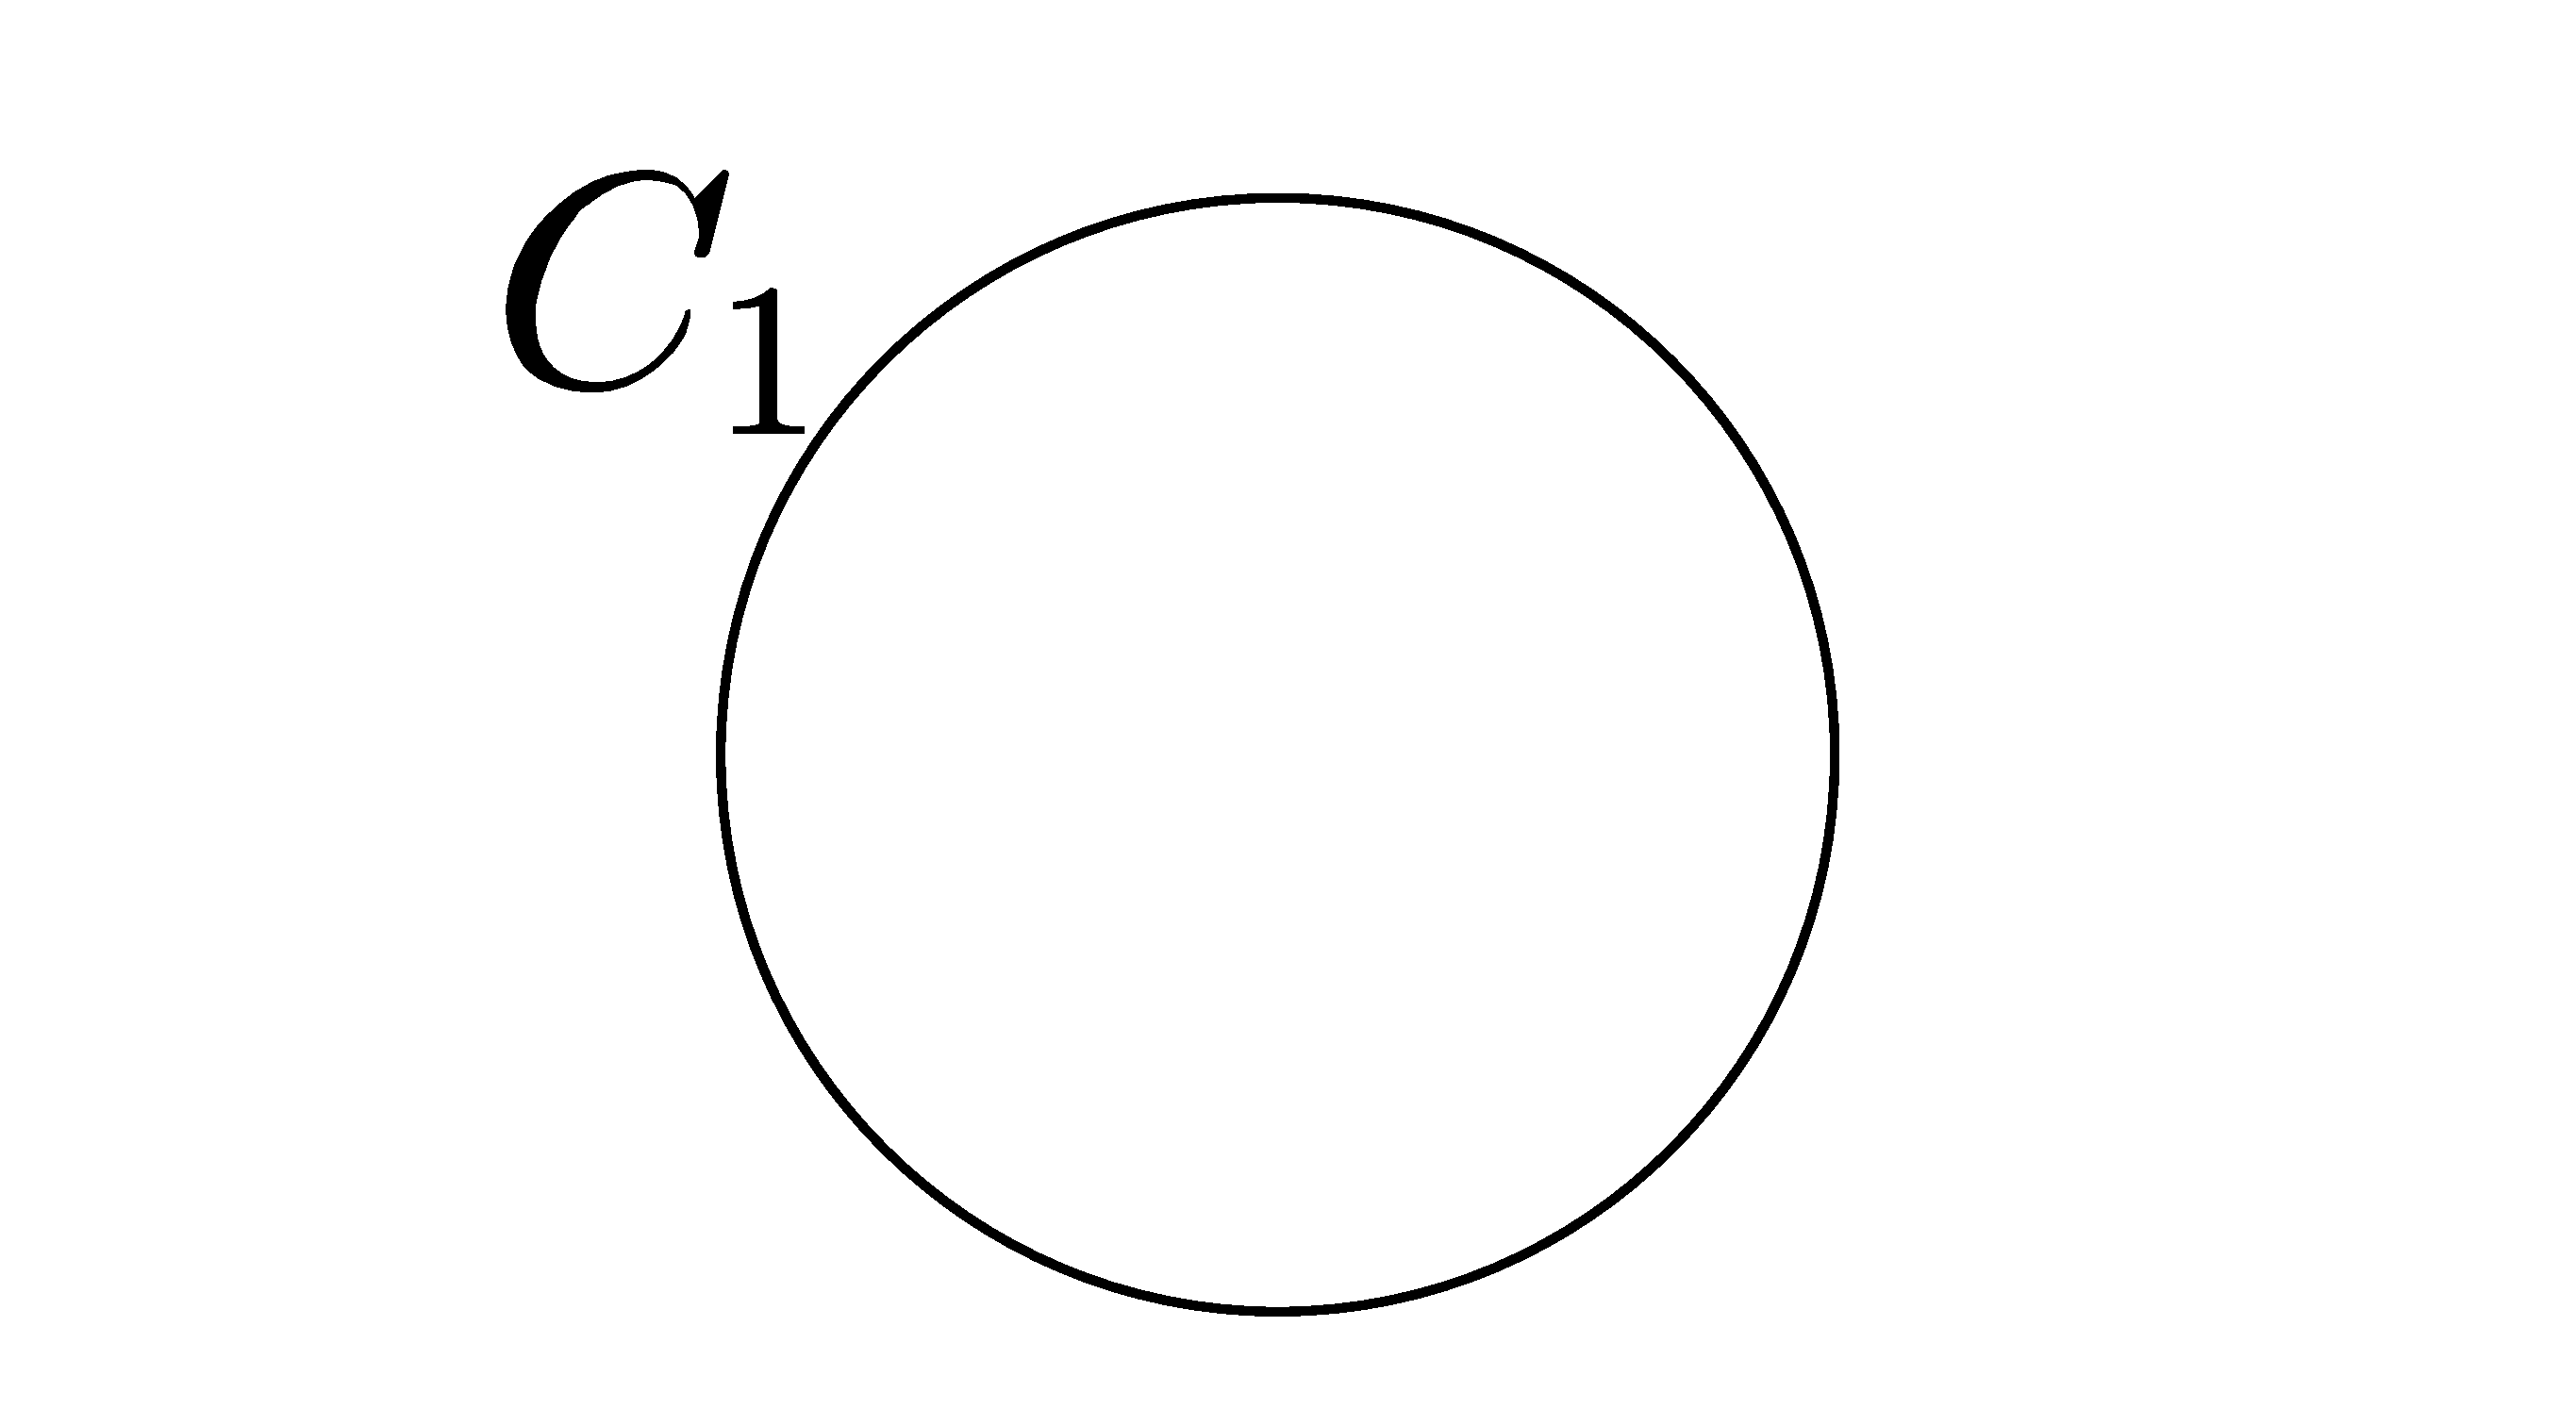
\includegraphics[scale=.065]{Graficos/elipse.eps}}
	\subfigure[Hipérbola]{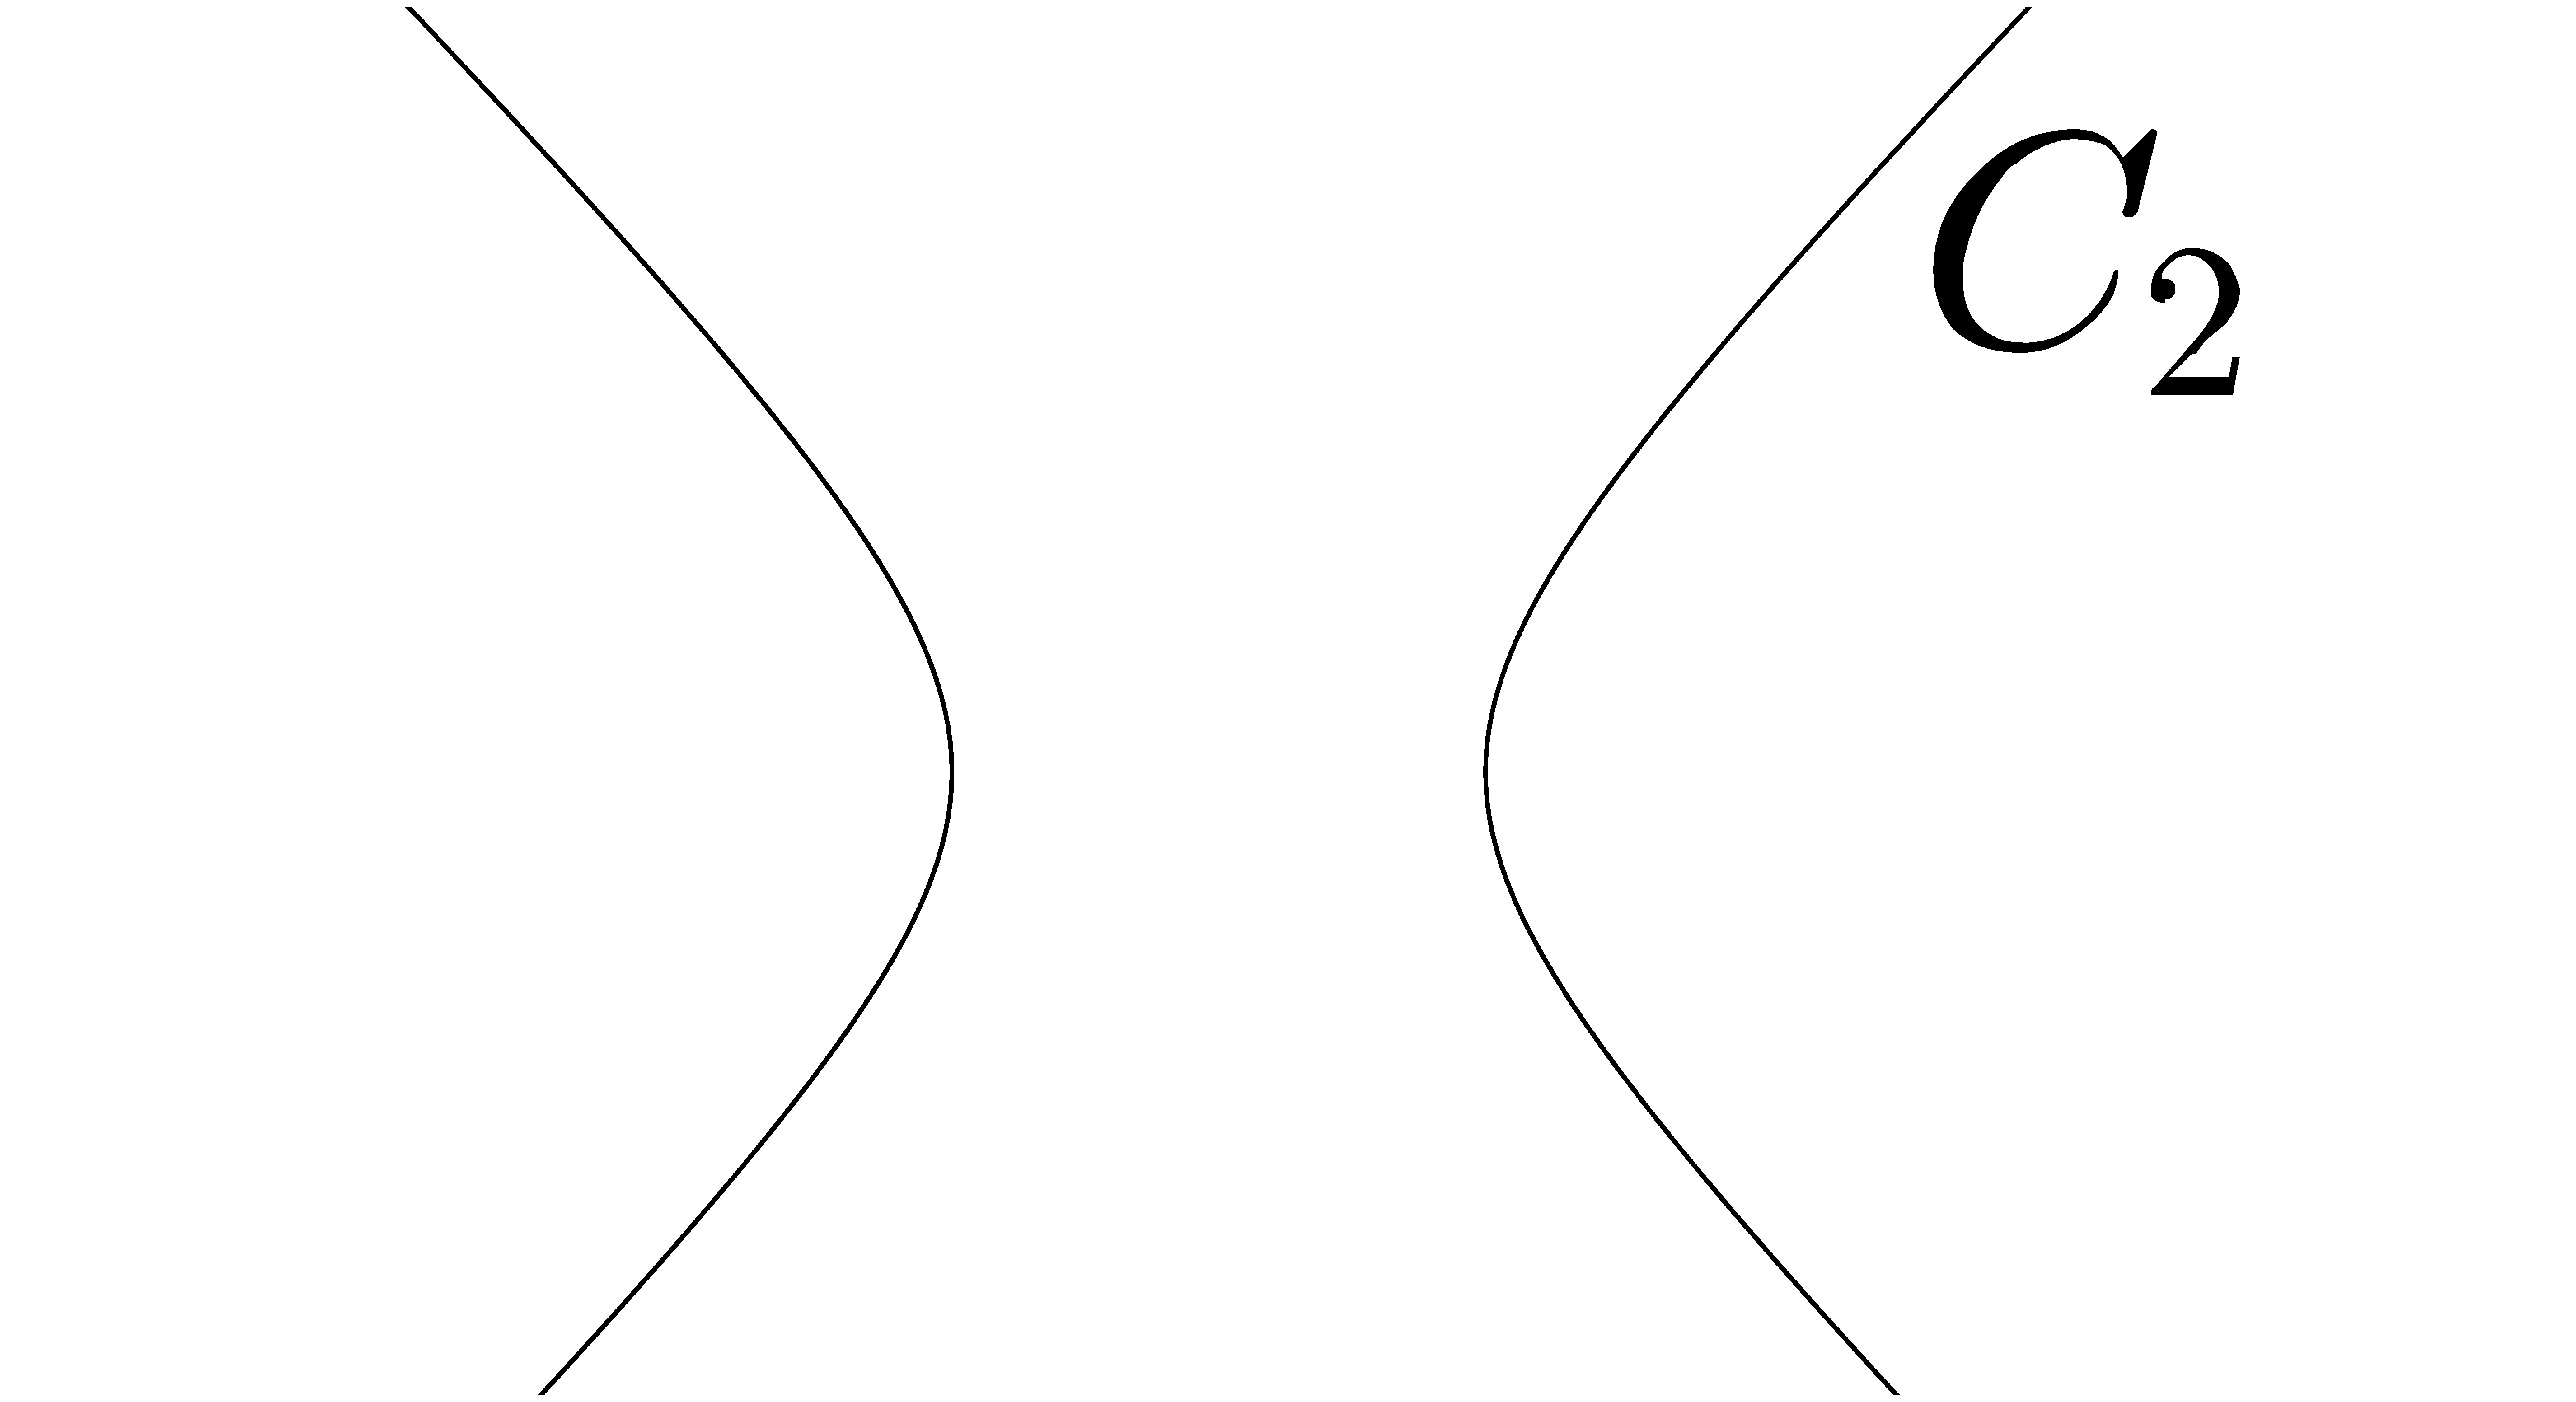
\includegraphics[scale=.028]{Graficos/hiperbola.eps}}
	\subfigure[Parábola]{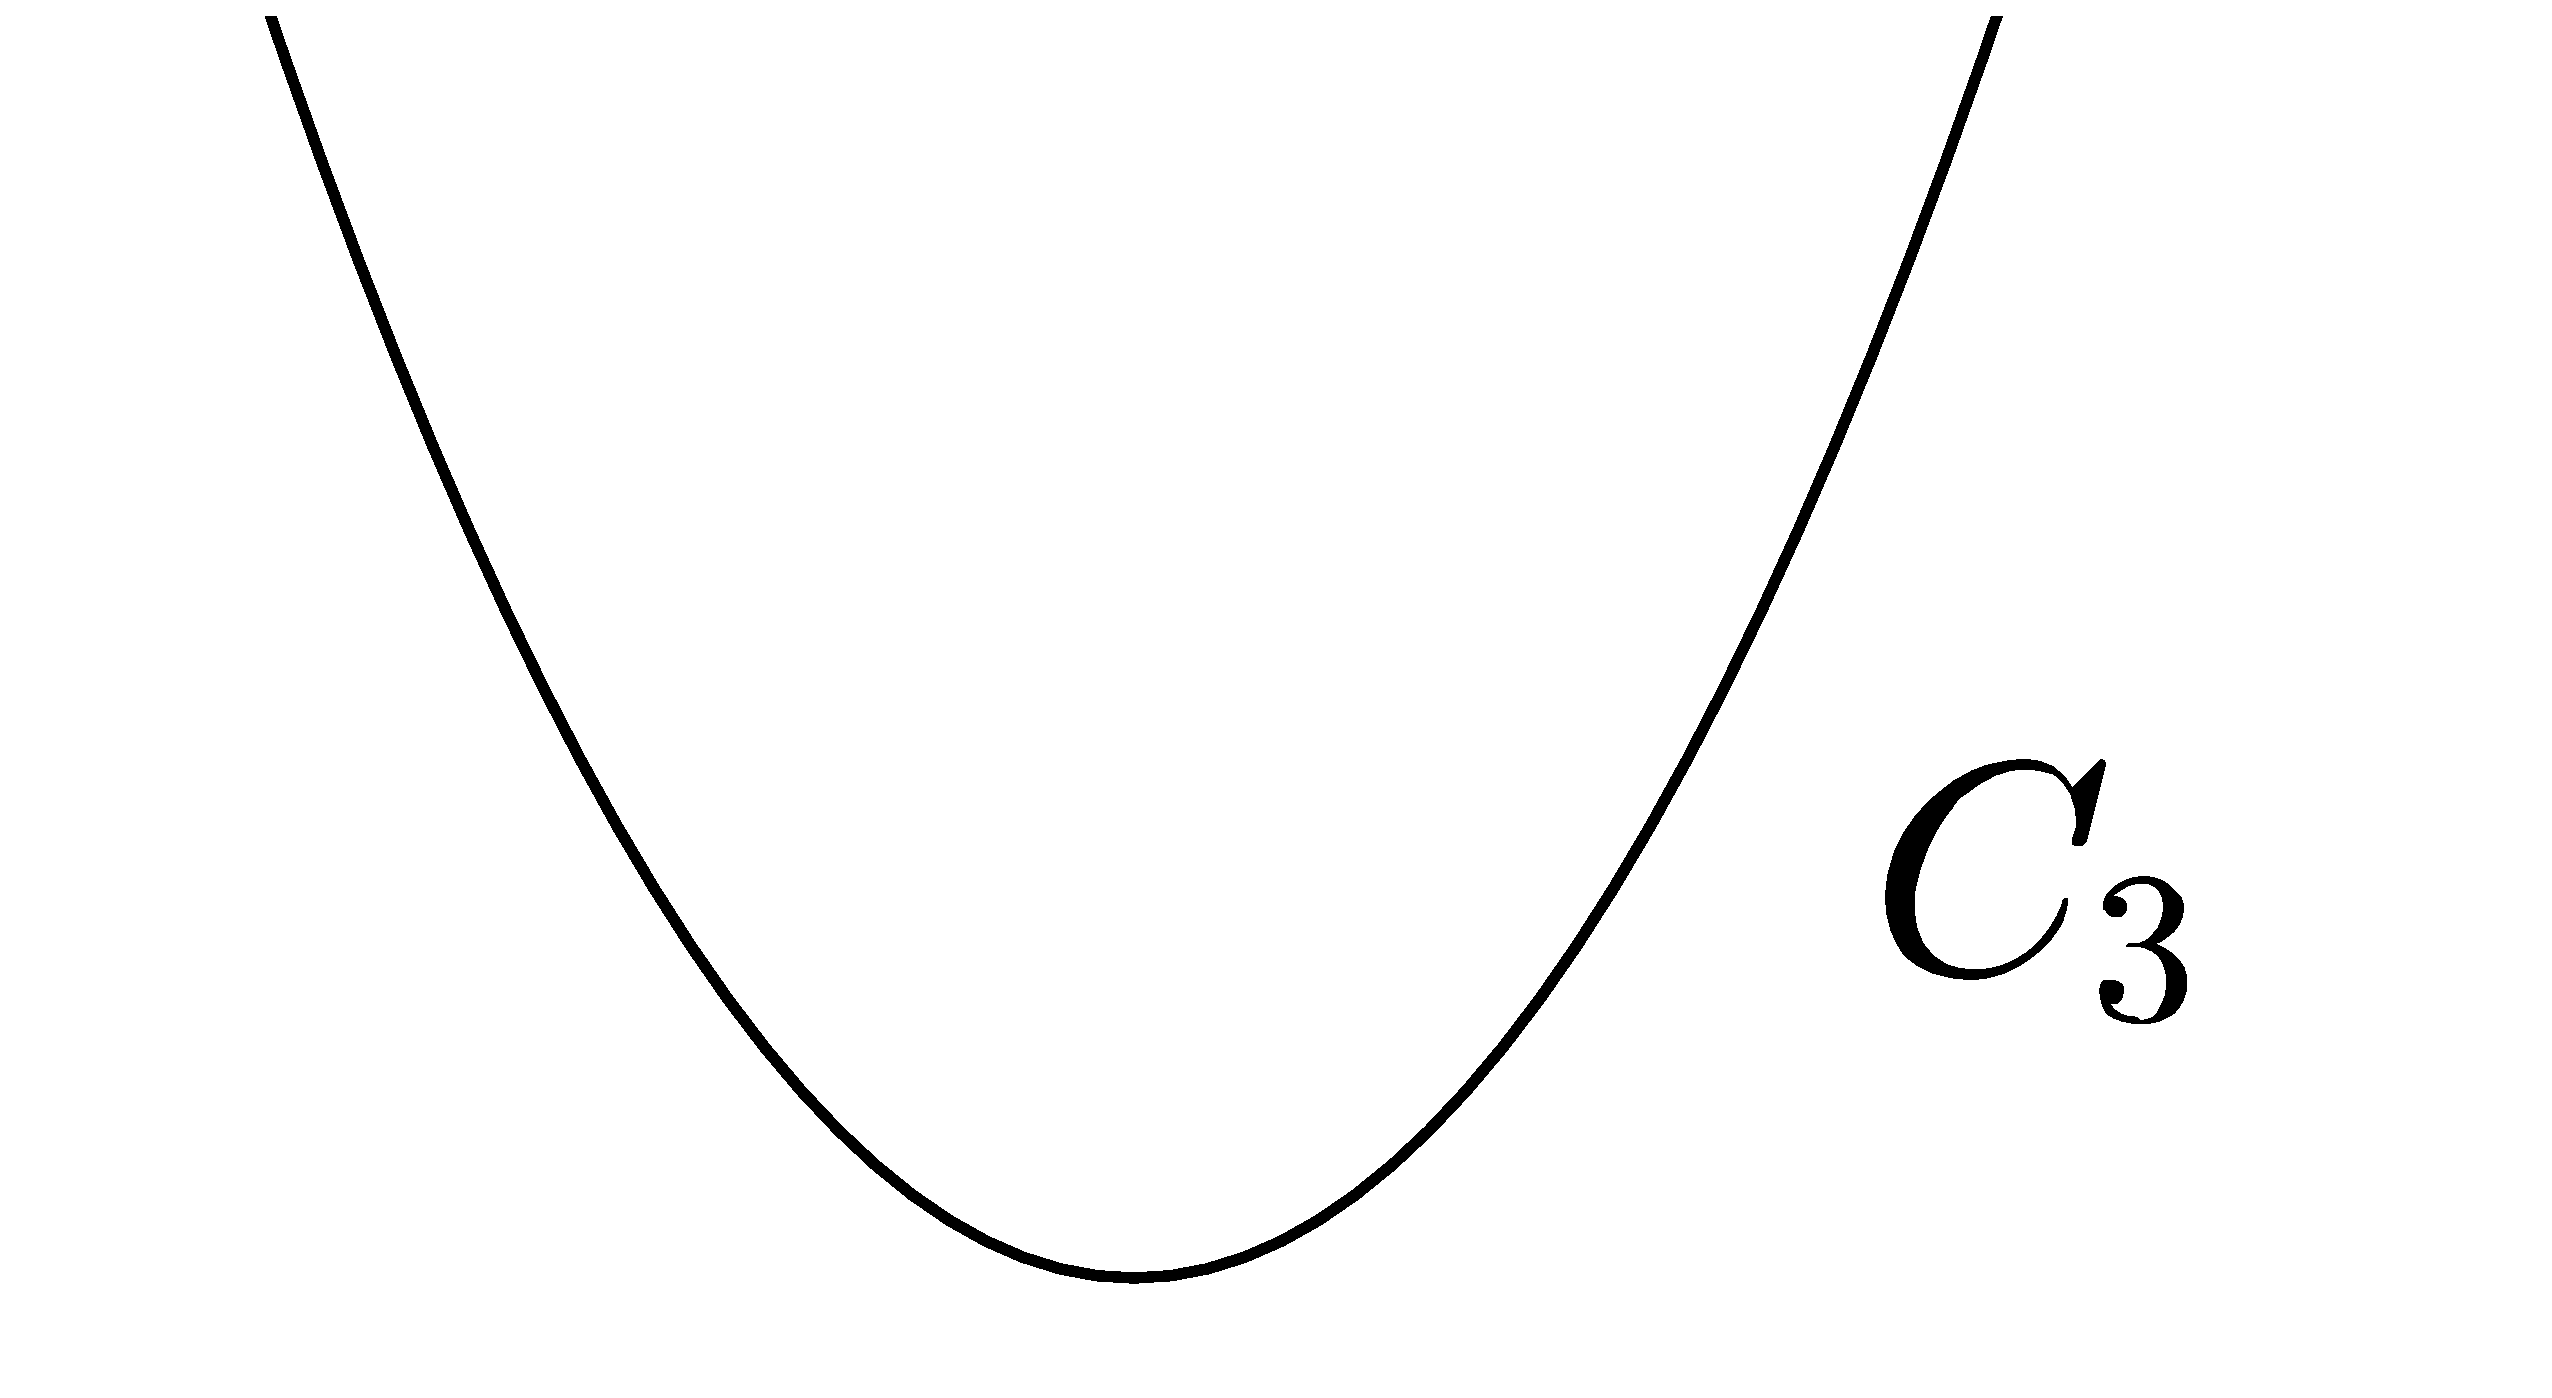
\includegraphics[scale=.06]{Graficos/parabola.eps}}
	\caption{Ilustración de los tipos de cónicas.}
	\label{C7_img_tiposConicas}
\end{figure}
Para que esta clasificación no resulte demasiado abstracta al lector, pongamos un ejemplos de cónicas de cada uno de los tipos.
\begin{exa}[Elipse]
	\label{C8_exa_elipse}
	Consideramos la cónica dada por la siguiente ecuación:
	\[C:x^2+y^2-z^2=0\]
	Intersequemos la cónica con la recta $l_\infty:z=0$ para poder clasificarla.
	\[\left.\begin{array}{c}
	x^2+y^2-z^2=0\\
	z=0
	\end{array}\right\}\leadsto x^2+y^2=0\]
	Es claro que la única solución a esta ecuación es el punto $(0,0,0)$, sin embargo, el rayo engendrado por este vector no está definido. Por ende, no hay ningún rayo (punto proyectivo) de la cónica que sea, a la vez, un rayo de la recta del infinito. Por ende, esta cónica es una elipse.
\end{exa}
\begin{exa}[Hipérbola]
	Clasifiquemos la cónica de ecuación:
	\[C:X^2-Y^2=1\]
	Antes de que cunda el pánico, nótese que esta ecuación nos viene dada en forma ``deshomogeneizada'' (si no no sería la ecuación de una cónica). Al homogeneizarla nos queda algo bastante más familiar:
	\[C:x^2-y^2-z^2=0\]
	Calculemos los puntos de corte con $z=0$:
	\[\left.\begin{array}{c}
	x^2-y^2-z^2=0\\
	z=0
	\end{array}\right\}\leadsto x^2=y^2\]
	Tomando raíces cuadradas y considerando todos los casos necesarios obtemos como soluciones los puntos de la forma:
	\[\begin{array}{cc}
	\class{(\lambda,\lambda,0)}=(1:1:0)\qquad & \qquad \class{(\lambda,-\lambda,0)}=(1:-1:0)
	\end{array}\]
	Por ende, la cónica $C$ tiene dos puntos de corte con la recta del infinito, esto significa que es de tipo hiperbólico.
\end{exa}
\begin{exa}[Parábola]
	Se nos da la siguiente cónica en forma no homogénea:
	\[C:Y=X^2\]
	Calculemos (tras homogeneizar) los puntos de corte de la misma con $l_\infty$.
	\[\left.\begin{array}{c}
	zy-x^2=0\\
	z=0
	\end{array}\right\}\leadsto x^2=0\]
	Teniendo en cuenta esto, los puntos que cumplen las restricciones impuestas por ambas ecuaciones son los de la forma $(0,\lambda,0)$ (los cuales, además, son solución doble). Estos generan un único rayo. Por ende, la cónica y la recta del infinito únicamente se cortan en un punto. Esto es lo mismo que decir que $C$ es una parábola.
\end{exa}
\section{Matriz de una Cuádrica}
Vamos a reescribir de una forma especialmente cómoda el polinomio asociado a una cónica. No es necesario memorizar como un loro el proceso de transformación que realizaremos a continuación, ya que, en breve, encontraremos una forma más rápida y simple de hacerlo.
\begin{multline}
	F(x,y,z)=ax^2+by^2+cz^2+2fyz+2gxz+2hxy=\\
	=x(ax+hy+gz)+y(by+fz+hx)+z(cz+fy+gx)
\end{multline}
Expresando todo esto e forma matricial obtenemos (compruébese):
\[F(x,y,z)=\begin{pmatrix}
x & y & z
\end{pmatrix}\begin{pmatrix}
ax+hy+gz\\
hx+by+fz\\
gx+fy+cz
\end{pmatrix}=\begin{pmatrix}
x & y & z
\end{pmatrix}\begin{pmatrix}
a & h & g\\
h & b & f\\
g & f & c
\end{pmatrix}\begin{pmatrix}
x\\
y\\
z
\end{pmatrix}\]
De forma abreviada (abusando de notación) usualmente escribiremos:
\[F(X)=X^tAX\]
A la matriz $A$ se la denomina \ti{matriz de la cónica} asociada al polinomio $F$. No mucho más adelante (simplemente por comodidad) desarrollaremos el concepto de \ti{matriz de una cuádrica} en general.

\begin{obs}[Matriz de una Cónica y Formas Bilineales]
	\label{C8_obs_bilineal}
	El lector que aún guarde en su mente bastantes remanentes de lo que cursó en su día de álgebra lineal se habrá dado cuenta de la relación entre el polinomio asociado a una cónica y las formas bilineales. De hecho, los polinomios asociados a cónicas \tb{son} formas bilineales simétricas. Además, lo que nosotros llamamos matriz de la cónica, es en realidad la matriz asociada a la forma bilineal.
	
	Sin embargo, una forma bilineal podía tener varias matrices asociadas (aunque solo una de ellas simétrica). Reflexionemos un poco sobre esto.
	
	Consideremos que la matriz $A$ es la asociada al polinomio $F$ (asociado a cierta cónica). Entonces, la imagen de un vector por el polinomio se escribe de la forma:
	\[F(X)=X^tAX\]
	Es ahora cuando traemos a colación un viejo y olvidado resultado de álgebra lineal que afirma que cualquier matriz puede ser descompuesta en una parte simétrica y otra antisimétrica de la siguiente manera:
	\[\begin{array}{ccc}
	A=A_s+A_a\qquad &\qquad A_s=\frac{1}{2}(A+A^t)\qquad &\qquad A_a=\frac{1}{2}(A-A^t)
	\end{array}\]
	En definitiva:
	\[F(X)=X^tAX=X^t(A_s+A_a)X=X^tA_sX+X^tA_aX\]
	Notemos que $X^tA_aX$ es un simple numeraco, luego coincide con su traspuesto:
	\[X^tA_aX=(X^tA_aX)^t=-X^tA_aX\sii X^tA_aX=0\]
	En conclusión, la parte antisimétrica de la matriz de una forma bilineal sólo introduce ruido y confusión. Ese es el motivo por el cual construimos (con una astucia en principio ajena al lector) una matriz simétrica como matriz de la cónica.
\end{obs}
Tras la observación \ref{C8_obs_bilineal} ya estamos en disposición de definir el concepto de \ti{matriz asociada a una cuádrica} como la matriz asociada a la forma bilineal simétrica que constituye su polinomio $F$ asociado.

Tras toda esta literatura, enunciemos y demostremos el prometido resultado que nos ayudaría a calcular de forma sencilla la matriz asociada a una cuádrica en general.
\begin{lem}[Matriz Asociada y Matriz Hessiana]
	\label{C8_lem_Hessiana}
	Dada una cuádrica $C$, su matriz asociada $A$ (simétrica) es única.

Además se tiene que: \[A=\frac{1}{2}\mathrm{Hess}(F)\]
Donde $F$ es el polinomio asociado a la cuádrica y $\mathrm{Hess}(F)$ su matriz Hessiana correspondiente.
\end{lem}
\begin{proof}
Demostremos en primer lugar el ``además'', obteniendo trivialmente el resto.

Consideremos el polinomio $F$ asociado a la cuádrica. Como vimos anteriormente, este polinomio admite la forma matricial:
\[F(X)=X^tAX\]
Nuestro objetivo es hallar una expresión única para los coeficientes $a_{ij}$ de la matriz $A$ de la cuádrica. Ayudados por el enunciado de nuestro problema (sabemos que nos tiene que salir la matriz Hessiana del polinomio $F$).

Para el lector que se haya saltado alguna clase de cálculo diferencial en varias variables, recordamos que la matriz Hessiana de una función $F:\C^n\to\C$ (en un punto genérico en el que admita derivadas parciales segundas) es:
\[\mathrm{Hess}(F)=\begin{pmatrix}
\frac{\partial F}{\partial x_1x_1} & \cdots &\frac{\partial F}{\partial x_nx_1}\\
\vdots & \ddots & \vdots\\
\frac{\partial F}{\partial x_1x_n} & \cdots & \frac{\partial F}{\partial x_nx_n}
\end{pmatrix}\]

Asimismo, cabe mencionar que si dicha función $F$ admite derivadas parciales segundas continuas en un punto, entonces la matriz Hessiana es simétrica. Esto es debido al llamado Teorema Mágico de Schwarz.

Para nuestra fortuna, los polinomios en general, y los polinomios asociados a cuádricas en particular, son funciones de clase infinito sobre todo su conjunto de definición, esto es, admiten derivadas parciales continuas de orden arbitrario en cualquier punto, luego su matriz Hessiana es siempre simétrica.

Hallemos pues un coeficiente arbitrario de la matriz Hessiana derivando dos veces $F$ respecto de las variables $x_i$ y $x_j$. Apoyándonos en la expresión matricial que tenemos, podemos ver el polinomio como el producto de dos matrices (matriz fila por matriz columna) que es fácilmente expresable como la siguiente suma (los corchetes son simplemente notacionales).
\[F(X)=(X^t)(AX)=\sum_{k=1}^{n}\left[x_k\left(\sum_{l=1}^{n}a_{kl}x_l\right)\right]\]
Derivando concuidado obtenemos:
\begin{multline}
	\frac{\partial F(x_1,\dots,x_n)}{\partial x_j\partial x_i}=\frac{\partial}{\partial x_j}\left(\frac{\partial F(x_1,\dots,x_n)}{\partial x_i}\right)=\\=\frac{\partial}{\partial x_j}\left(\sum_{k\not= i}^{n}\left[x_k\frac{\partial}{\partial x_i}\left(\sum_{l=1}^{n}a_{kl}x_l\right)\right]+\left(\sum_{l=1}^{n}a_{il}x_l+x_ia_{ii}\right)\right)=\\
	=\frac{\partial}{\partial x_j}\left(\sum_{k\not=i}^{n}x_ka_{ki}+x_ia_{ii}+\sum_{l=1}^{n}a_{il}x_l\right)=\\=\frac{\partial}{\partial x_j}\left(\sum_{k=1}^{n}x_ka_{ki}+\sum_{l=1}^{n}a_{il}x_l\right)=a_{ji}+a_{ij}=2a_{ij}
\end{multline}
Por ende, cada coeficiente de la matriz Hessiana es el doble del coeficiente correspondiente de la matriz de la cuádrica.

Como las derivadas parciales son, al fin y al cabo, límites, estas son únicas, luego la matriz de una cuádrica es única. Además, de esta forma, tenemos un procedimiento efectivo y mecánico para calcularla.
\end{proof}
Pongamos algún ejemplo para que el lector ponga en valor la utilidad de la caracterización ofrecida por el lema \ref{C8_lem_Hessiana}.
\begin{exa}[Cálculo de la Matriz de una Cuádrica]
	Dadas las siguientes cónicas, calculemos automáticamente sus matrices asociadas obteniendo la mitad de las matrices Hessianas de los polinomios.
	\[\begin{array}{c}
	C_1:x^2+y^2+z^2=0\leadsto\frac{1}{2}\begin{pmatrix}
	1 & 0 & 0\\
	0 & 1 & 0\\
	0 & 0 & 1
	\end{pmatrix}\\
	C_2:x^2+y^2+2z^2=0\leadsto\frac{1}{2}\begin{pmatrix}
	1 & 0 & 0\\
	0 & 1 & 0\\
	0 & 0 & 2
	\end{pmatrix}
	\end{array}\]
\end{exa}
A continuación veremos que dos polinomios ``proporcionales'' generan la misma cuádrica.

Esto es importante por muchos motivos. El primero, y el más evidente a simple vista, es que para calcular la matriz de una cuádrica ya no hace falta multiplicar la matriz Hessiana del polinomio $F$ por ningún factor. Bastaría considerar que la cuádrica está generada por el polinomio $2F$. Veamos esto con detalle.
\begin{obs}[Polinomios Proporcionales]
	\label{C8_obs_proporcionales}
	Dado un polinomio $F$ (con las restricciones habituales), resulta evidente que el conjunto de ceros de $F$ es igual al conjunto de ceros del polinomio $\lambda F$ para cierto $\lambda\in\C$ no nulo.
\end{obs}
Otro de los motivos por los que la observación \ref{C8_obs_proporcionales} es de gran importancia, es que, como veremos (dejándonos pendiente algún detalle), el conjunto de las cúadricas proyectivas de $\proy(\C^n)$ puede verse como un espacio proyectivo $\proy(\C^k)$ para cierto $k$ (que calcularemos explícitamente). 
\begin{obs}[Pseudolema de la Correspondencia]
	\label{C8_obs_pseudoCorrespondencia}
	Es evidente que la relación de proporcionalidad de polinomios es una relación de equivalencia a la que denotaremos $\sim$. Consideremos pues el conjunto cociente de los polinomios (compuestos únicamente por monomios de grado $2$, a los que denotaremos por $\mc{P}$) ``módulo'' la relación de equivalencia $\sim$. A este conjunto lo denotaremos:
	\[\mc{F}:=\frac{\mc{P}}{\sim}\]
	Es una fácil comprobación (que se deja al lector) demostrar que el conjunto de los polinomios con nuestras restricciones habituales es un espacio vectorial (cuya dimensión desconocemos por el momento). Por ello, el conjunto $\mc{F}$ no es más que el espacio proyectivo asociado a $\mc{P}$. Por este motivo, denotaremos por $\class{F}$ a los elementos de $\mc{F}$.
	
	Es evidente (por definición) que la siguiente aplicación es sobreyectiva:
	\[\begin{array}{c}
	\mc{F}\stackrel{\Psi}{\to}\mc{C}\\
	\class{F}\mapsto\phi(F)
	\end{array}\]
	Donde $\mc{C}$ representa el conjunto de las cuádricas del espacio proyectivo complejo $n+1$ dimensional y $\phi$ es la aplicación que a cada polinomio le asocia su conjunto de ceros.
	
	Resulta ser también cierto (como veremos más adelante) que la aplicación $\Psi$ es inyectiva, pudiendo identificar canónicamente al conjunto de cuádricas $\mc{C}$ con el espacio proyectivo $\mc{F}$.
\end{obs}
	Hagamos un pequeño (gran) acto de fe y consideremos probado que la aplicación $\Psi$ definida en la observación \ref{C8_obs_pseudoCorrespondencia} es (como ya se adelantó) biyectiva. Dando esto por hecho, tratemos de calcular la dimensión de $\mc{P}$.
	\begin{obs}[Dimensión de $\mc{P}$]
		\label{C8_obs_dimension}
		Como ya sabemos, los vectores de $\mc{P}$ son formas bilineales simétricas, y como tales, quedan totalmente determinadas por una matriz simétrica $n\times n$. Es un ejercicio de álgebra lineal comprobar que la aplicación que asociada a cada polinomio $F$ su matriz correspondiente es un isomorfismo de espacios vectoriales.
		
		Esto quiere decir que $\mc{P}$ y el espacio vectorial de las matrices simétricas $n\times n$ tienen la misma dimensión, que es, precisamente, (compruébese) $\frac{n^2+n}{2}:=\xi$.
		
		Por ende, $\mc{P}$ es isomorfo a $\C^\xi$. Como las cuádricas de $\C^n$ se confunden con $\proy(\mc{P})\cong\proy(\C^\xi)$, habitualmente se dirá que las cuádricas de $\C^n$ \ti{son} un $\proy(\C^\xi)$.
	\end{obs}
	\begin{obs}[Las cónicas \ti{son} un $\proy^5$]
		Un resultado cuanto menos sorprendente, y bonito, que se desprende de forma inmediata de la observación \ref{C8_obs_dimension}, es que las cónicas del plano proyectivo complejo son un espacio proyectivo de dimensión $5$. En efecto:
		\[\xi=\frac{3^2+3}{2}-1=5\]
		No debemos olvidarnos de que queda pendiente la demostración de que cada cuádrica está asociada a un único rayo de polinomios.
	\end{obs}
Recapitulemos. A lo largo de esta sección hemos aprendido que todo rayo de polinomios está asociado a una cuádrica. Además, sabemos que ser un punto de una cúadrica $C$ significa verificar la ecuación matricial de dicha cuádrica. Es decir:
\[x\in C\sii X^t\mathrm{Hess}(F)X=0\] 
\section{Determinaciones de una Cónica}
El objetivo de esta sección será demostrar que, bajo ciertas condiciones, cinco puntos del espacio proyectivo $\proy^2$ determinan unívocamente una cónica.
\subsection{Cónicas como Producto de dos Rectas}
Dadas dos rectas de $\proy^2$, a las que $l$
\section{Deshomogeneizaciones de una Cónica}